\documentclass[11pt,a4paper]{article}

\usepackage[T1]{fontenc}
\usepackage[utf8]{inputenc}
\usepackage{lmodern}
\usepackage[margin=2.4cm]{geometry}
\usepackage{booktabs}
\usepackage{graphicx}
\usepackage{float}
\usepackage{caption}
\usepackage{hyperref}
\usepackage{amsmath}
\usepackage{array}
\usepackage{enumitem}

\captionsetup{font=small,labelfont=bf}
\graphicspath{{figures/}}
\setlist[itemize]{topsep=2pt,itemsep=2pt,parsep=0pt}
\setlength{\emergencystretch}{2em}

\title{UPA Project 2\\Exploratory Analysis and Data Preparation\\for Flashlight Price Prediction}
\author{Team xrepcim00\\Solvers: xrepcim00, xvesela00}
\date{\today}

\begin{document}

\maketitle
\tableofcontents
\clearpage

\section{Introduction and dataset description}

This report documents the exploratory analysis and the data preparation performed
on the dataset created in the first part of the project. The dataset was collected
from the flashlight category of the foreign e-shop
\href{https://www.knivesandtools.com/en/ct/flashlights.htm}{knivesandtools.com}.
It contains 200 products. The raw TSV file has no header and contains nine
attributes: product URL, product name, current selling price in EUR, brand,
colour, length, weight, material and maximum light intensity in lumens.

All values were originally stored as strings. The analysis loader converts
length, weight, price and lumens to numbers, splits colour and material into
lists, and derives four binary flags from the product name:
\texttt{rechargeable}, \texttt{tactical}, \texttt{edc} and \texttt{bundle}.
The resulting dataframe has 200 rows and 13 columns (the nine raw attributes
plus the four derived flags).

The selected mining task is supervised \textbf{price prediction}. Two prepared
datasets are created: one for algorithms that require categorical inputs
(price classification) and one for algorithms that require numeric inputs
(price regression). The target is the current selling price, it is not used as
a predictor in the preparation pipeline.

\subsection{Dataset overview}

Table~\ref{tab:overview} summarises the attributes, their data types, the number
of non-missing values and the number of distinct values. For list-valued
attributes, a list is counted as one value.

\begin{table}[H]
\centering
\small
\caption{Dataset attributes and basic characteristics.}
\label{tab:overview}
\begin{tabular}{llrr}
\toprule
Attribute & Type & Non-missing & Distinct \\
\midrule
url & string & 200 & 200 \\
name & string & 200 & 200 \\
price & numeric & 200 & 129 \\
brand & categorical & 200 & 7 \\
colour & list of strings & 200 & 22 \\
length\_cm & numeric & 194 & 96 \\
weight\_g & numeric & 199 & 106 \\
material & list of strings & 196 & 11 \\
lumens & numeric & 197 & 74 \\
rechargeable & binary & 200 & 2 \\
tactical & binary & 200 & 2 \\
edc & binary & 200 & 2 \\
bundle & binary & 200 & 2 \\
\bottomrule
\end{tabular}
\end{table}

The numeric attributes are summarised in Table~\ref{tab:numeric}. All four are
strongly right-skewed. The median price is about 80 EUR, while the maximum is
almost 581 EUR. The median brightness is 1,200 lumens, while the maximum is
21,000 lumens. The mean is substantially larger than the median for price,
weight and brightness, which confirms the long right tails.

\begin{table}[H]
\centering
\small
\caption{Numeric attribute summary.}
\label{tab:numeric}
\begin{tabular}{lrrrrrrr}
\toprule
Attribute & Count & Mean & Std. & Min & 25\,\% & 50\,\% & 75\,\% \\
\midrule
price & 200 & 106.17 & 86.49 & 16.99 & 56.99 & 79.99 & 120.12 \\
length\_cm & 194 & 14.43 & 5.34 & 3.50 & 12.10 & 14.00 & 15.50 \\
weight\_g & 199 & 188.13 & 227.47 & 24.00 & 72.00 & 126.00 & 203.00 \\
lumens & 197 & 2336.70 & 3385.68 & 9.00 & 400.00 & 1200.00 & 3000.00 \\
\bottomrule
\end{tabular}
\end{table}

The maximum values are 580.95 EUR, 43.4 cm, 1,636 g and 21,000 lumens,
respectively. These are not necessarily errors, they correspond to large
professional searchlights and large D-cell torches.

\subsection{Most frequent categorical values}

The brand distribution is dominated by Fenix (62 products), Nitecore (45) and
Maglite (31). Ledlenser and Wuben have 25 products each, Streamlight has 11 and
HDS systems has a single product. Black is by far the most common colour (155
products), followed by grey (11) and green (10). Aluminum is the dominant
material (170 products). Plastic (17), polycarbonate (7), stainless steel (6)
and composite (5) are less frequent. A product can list more than one colour or
material, the counts above count every mentioned value.

The derived flags are also informative: 106 products are rechargeable, 37 are
described as tactical, 35 as EDC (everyday carry) and 8 are bundle/accessory
listings. These flags are binary and are included as features in both prepared
variants. The bundle flag marks kits, packs, holsters, cables, battery systems
and listings with attachments, it does not remove those products.

\section{Exploratory analysis}

\subsection{Distribution of values}

Figure~\ref{fig:price} compares the raw and logarithmic price distributions.
The linear histogram has a long right tail: most products cost between roughly
30 and 150 EUR, while a small number of professional searchlights cost more than
350 EUR. On the logarithmic scale the distribution is closer to symmetric,
which justifies the log transformation used in the numeric variant.

\begin{figure}[H]
\centering
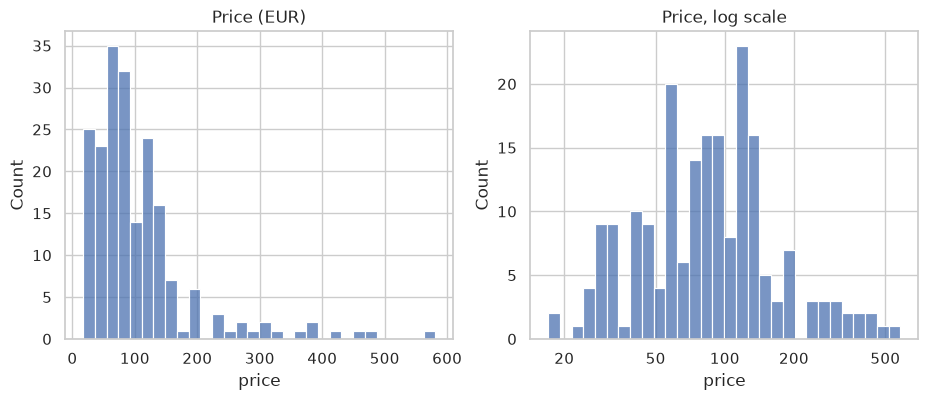
\includegraphics[width=\linewidth]{fig1_price_distribution.png}
\caption{Distribution of product prices: linear scale (left) and logarithmic
scale (right).}
\label{fig:price}
\end{figure}

Figure~\ref{fig:brand} shows the price distribution by brand. Fenix and Nitecore
have the widest ranges and several high-priced products. Maglite is concentrated
at the lower end of the market. Ledlenser and Wuben occupy the middle. The single
HDS systems product is a premium item and its box is not representative, so the
brand is grouped into \texttt{other} during preparation.

\begin{figure}[H]
\centering
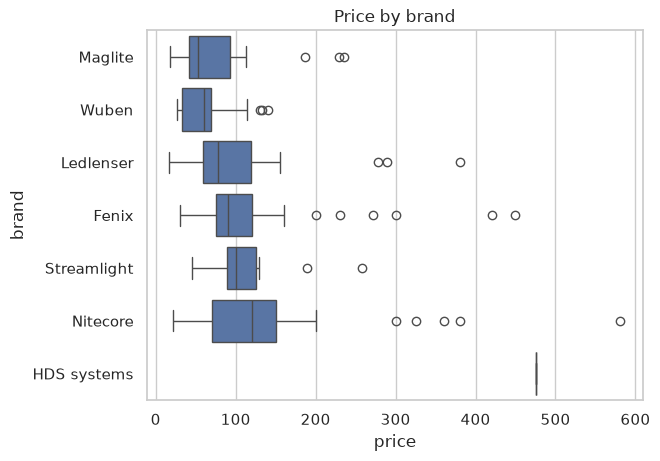
\includegraphics[width=0.9\linewidth]{fig2_price_brand_box.png}
\caption{Price distribution by brand.}
\label{fig:brand}
\end{figure}

Figure~\ref{fig:lumens} relates price to maximum brightness. Both axes use a
logarithmic scale because both attributes span several orders of magnitude.
Price and brightness are positively related, but the relationship is not
deterministic. At a given brightness, rechargeable models tend to be slightly
more expensive, which is consistent with the additional electronics and battery.
The plot also exposes the high-brightness products with 4,000--21,000 lumens,
these are the main source of the heavy tail in both attributes.

\begin{figure}[H]
\centering
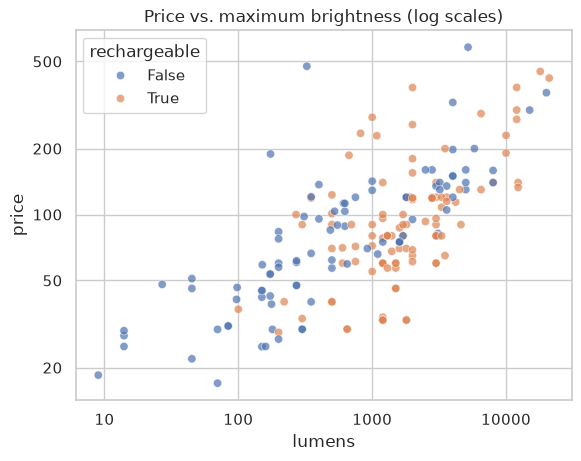
\includegraphics[width=0.85\linewidth]{fig3_price_lumens_scatter.png}
\caption{Price versus maximum brightness, coloured by rechargeability.}
\label{fig:lumens}
\end{figure}

Figure~\ref{fig:material} counts the materials mentioned by the products.
Aluminum is by far the most common material, followed by plastic and
polycarbonate. The long tail contains stainless steel, composite, rubber,
carbon fibre, polymer and nylon. Because several materials occur only a few
times, rare materials are grouped into \texttt{other} in the prepared datasets.

\begin{figure}[H]
\centering
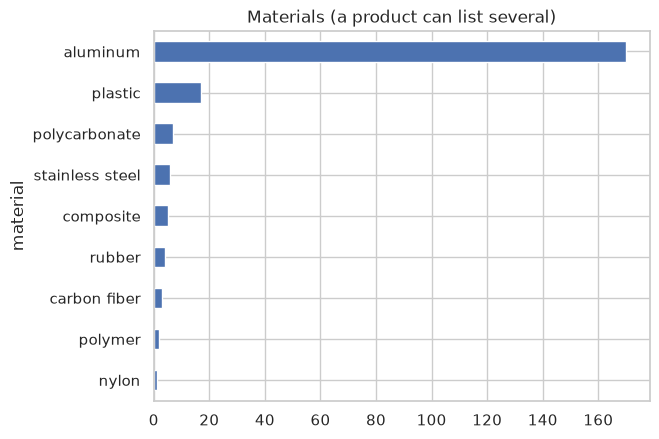
\includegraphics[width=0.8\linewidth]{fig4_materials_bar.png}
\caption{Materials mentioned by the products. A product can list several
materials.}
\label{fig:material}
\end{figure}

Figure~\ref{fig:violin} combines the brand comparison with rechargeability.
The two halves of each violin show the price distribution for non-rechargeable
and rechargeable products. Rechargeability changes the distribution mainly for
Fenix and Nitecore, for Maglite the two halves are much closer because most
Maglite products are traditional battery-powered torches. The overlap between
brands also shows that brand alone does not separate price classes.

\begin{figure}[H]
\centering
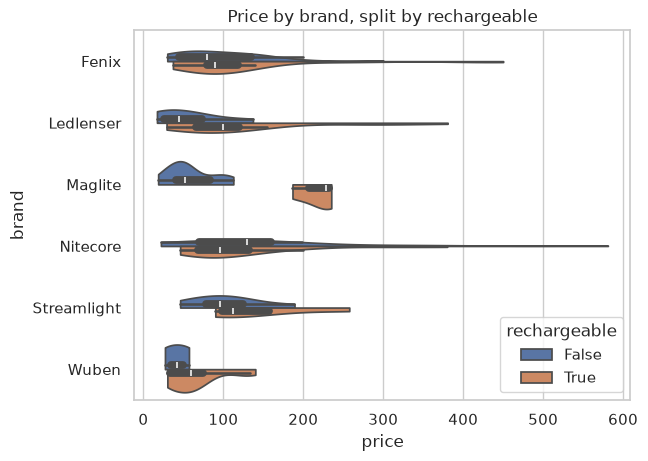
\includegraphics[width=0.85\linewidth]{fig5_price_brand_violin.png}
\caption{Price by brand, split by rechargeability.}
\label{fig:violin}
\end{figure}

Figure~\ref{fig:box} compares the ranges and quartiles of all numeric
attributes. Every attribute has observations above the upper whisker.
Weight and brightness have the most extreme tails, while length is dominated by
compact products and a few large D-cell torches. The figure also motivates the
IQR outlier detection described in the next section.

\begin{figure}[H]
\centering
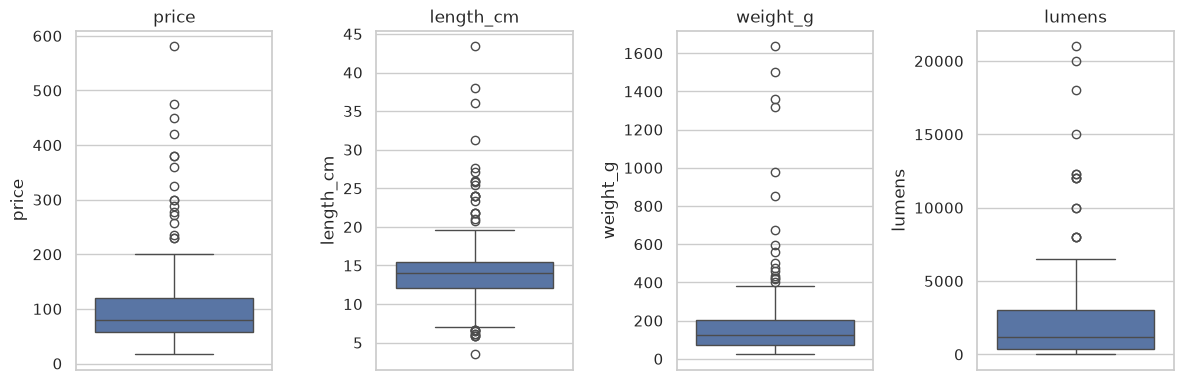
\includegraphics[width=\linewidth]{fig6_numeric_boxplots.png}
\caption{Boxplots of the four numeric attributes.}
\label{fig:box}
\end{figure}

\subsection{Outlier analysis}

Outliers were detected with two methods:

\begin{itemize}
  \item the IQR rule: a value is an outlier if it is below
        \(Q_1 - 1.5\,\mathrm{IQR}\) or above \(Q_3 + 1.5\,\mathrm{IQR}\),
  \item the standard z-score: \(|z| > 3\).
\end{itemize}

The results are shown in Table~\ref{tab:outliers}. The IQR rule marks 48
products in at least one attribute, while the z-score marks 12 products.

\begin{table}[H]
\centering
\small
\caption{Number of detected outliers per attribute and method.}
\label{tab:outliers}
\begin{tabular}{lrr}
\toprule
Attribute & IQR & z-score \\
\midrule
price & 17 & 6 \\
length\_cm & 31 & 4 \\
weight\_g & 16 & 5 \\
lumens & 14 & 4 \\
\midrule
any attribute & 48 & 12 \\
\bottomrule
\end{tabular}
\end{table}

The differences between the methods are expected. The IQR rule is sensitive to
a larger number of moderately extreme values, whereas the z-score is dominated
by the very largest observations. The 12 products flagged by the z-score
include, for example, the Fenix LR60R (21,000 lumens, 419.99 EUR), the Fenix
LR80R (18,000 lumens, 449.95 EUR), the Nitecore TM39 (580.95 EUR), the
Ledlenser P21R (12,000 lumens) and the Maglite 5-D torch (43.4 cm, 596 g).
These are valid premium or large products, not data-entry errors.

Because these products are valid, they were not deleted, capped or otherwise
altered in the prepared datasets. Their influence is reduced by quantile
discretization in variant A and by a logarithmic transformation in variant B.
Section~\ref{sec:prep} discusses the alternative methods that could be used if
the extremes were known to be measurement errors.

\subsection{Missing values}

The dataset contains 14 missing values in total, which is about 0.8\,\% of all
cells. Table~\ref{tab:missing} shows the distribution by attribute and by
product.

\begin{table}[H]
\centering
\small
\caption{Missing values by attribute and by product.}
\label{tab:missing}
\begin{tabular}{lr}
\toprule
Item & Count \\
\midrule
length\_cm & 6 \\
material & 4 \\
lumens & 3 \\
weight\_g & 1 \\
\midrule
total missing cells & 14 \\
products with 0 missing values & 189 \\
products with 1 missing value & 9 \\
products with 2 missing values & 1 \\
products with 3 missing values & 1 \\
\bottomrule
\end{tabular}
\end{table}

The two products with more than one gap are the Nitecore TM20K (missing length
and material) and a Nitecore 21700 battery accessory (missing length, material
and lumens). The remaining gaps are isolated. The missingness is not
systematic enough to justify deleting rows. Imputation is therefore preferable,
two different approaches are used in the two prepared variants.

\subsection{Correlation analysis}

Figure~\ref{fig:corrnum} shows Pearson and Spearman correlation matrices for the
numeric attributes.

\begin{figure}[H]
\centering
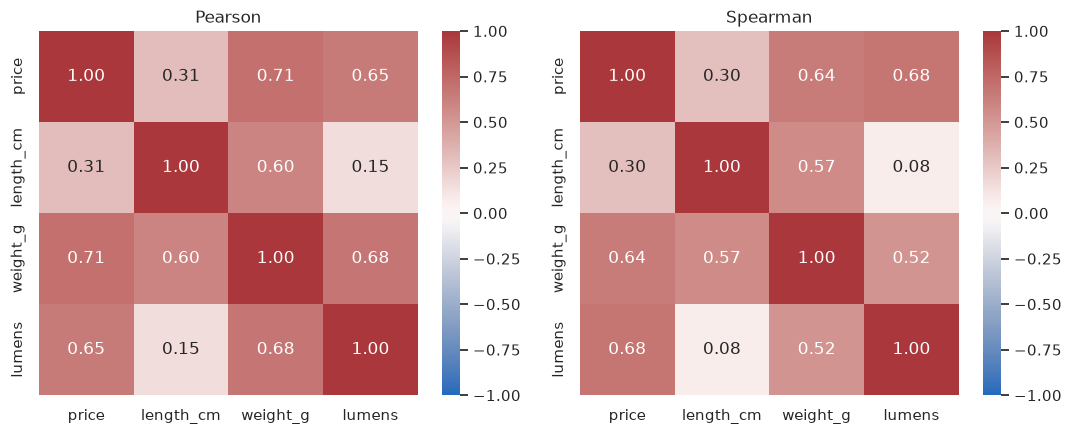
\includegraphics[width=\linewidth]{fig7_correlation_numeric.png}
\caption{Pearson (left) and Spearman (right) correlations of numeric
attributes.}
\label{fig:corrnum}
\end{figure}

Weight and brightness are the strongest correlates of price. The Pearson
coefficients are 0.710 for weight and 0.651 for brightness, the corresponding
Spearman coefficients are 0.643 and 0.682. Length is a weaker correlate
(Pearson 0.312, Spearman 0.303). Weight and brightness are also correlated with
each other (Pearson 0.675, Spearman 0.521), so a model should not rely on a
single attribute. Length and brightness are almost uncorrelated in the
Spearman matrix (0.077), despite both being related to price. These results are
descriptive, they do not imply causality.

\section{Data preparation for mining}
\label{sec:prep}

\subsection{Mining task and attribute selection}

The task is to predict the current selling price. Two variants are prepared so
that the same problem can be solved by algorithms with different input
requirements:

\begin{itemize}
  \item variant A: price classification into \texttt{low}, \texttt{mid} and
        \texttt{high} classes, with all predictors discretized,
  \item variant B: price regression, with categorical attributes encoded as
        binary columns and numeric attributes normalized.
\end{itemize}

The attributes \texttt{url} and \texttt{name} are identifiers and are removed.
The four flags derived from the name are kept because they describe product
type, in particular, the \texttt{bundle} flag marks kits, packs, holsters,
cables, battery systems and listings with attachments. \texttt{colour}
is dropped because it is almost constant: 155 of the 200 products list
black as a colour, so the attribute carries little information for this sample.
\texttt{material} is retained. It can contain several
comma-separated values, the first listed value is used as the primary value,
and rare categories (fewer than five products) are grouped into \texttt{other}.
This simplification keeps the table compact while preserving the most important
materials.

\subsection{Missing-value handling}

Two different imputation strategies are used, as required by the assignment.

\paragraph{Variant A.} Missing numeric predictors are replaced by the median of
the product's brand. This preserves brand-specific scale: for example, Maglite
torches are generally longer and heavier than keychain lights. Missing
categorical values are replaced by the most common value of the attribute.
Group-wise median imputation is simple, interpretable and robust to the small
number of gaps. The mode is a natural choice for categorical attributes with a
dominant category.

\paragraph{Variant B.} Missing categorical values are kept as an explicit
\texttt{unknown} category. Missing numeric predictors are imputed with a
5-nearest-neighbour (KNN) imputer after the predictor columns have been scaled.
KNN can exploit similarities between products and is therefore less coarse than
a single global median. The imputer is fitted only on the predictor matrix, the
price target is excluded from the distance calculation and is attached after
imputation. This prevents target leakage, which would occur if the price were
known during imputation but unknown at prediction time.

\subsection{Outliers in the prepared datasets}

The outliers identified in Section 2.2 are valid premium or large products, so
no values or rows were removed or capped. Variant A is
naturally robust because quantile discretization assigns the largest values to
the high bin, the equal-frequency construction limits their influence on the
class distribution. Variant B applies
\(\log(1+x)\) to the numeric predictors before min--max normalization, this
compresses the long right tails and reduces the leverage of extreme values.

If the extremes had been data errors, several alternatives could be used:
winsorization at the IQR fences, capping at the 1st/99th percentile, deletion of
the affected rows, or an explicit outlier indicator. These methods were not
applied because the extremes are genuine products and removing them would bias
the dataset towards cheaper, smaller models. The residual influence of the
outliers is a documented limitation of variant B.

\subsection{Variant A: categorical dataset}

Variant A uses the following steps:

\begin{enumerate}
  \item remove the identifier columns and group rare categories,
  \item replace missing numeric predictors with the brand median,
  \item replace missing categorical values with the attribute mode,
  \item discretize every numeric attribute, including the target, into three
        quantile-based bins (\texttt{low}, \texttt{mid}, \texttt{high}),
  \item convert the binary flags to \texttt{yes}/\texttt{no}.
\end{enumerate}

Quantile discretization was chosen because it produces approximately balanced
classes and is robust to the remaining skew. The resulting price classes contain
67 low, 66 mid and 67 high products. The output file is
\texttt{data\_categorical.csv} with 200 rows and 10 columns:
\texttt{price}, \texttt{brand}, \texttt{length\_cm}, \texttt{weight\_g},
\texttt{material}, \texttt{lumens}, \texttt{rechargeable}, \texttt{tactical},
\texttt{edc} and \texttt{bundle}. All columns are categorical, so the file is
suitable for algorithms that require categorical inputs.

\subsection{Variant B: numeric dataset}

Variant B uses the following steps:

\begin{enumerate}
  \item remove the identifier columns and group rare categories,
  \item replace missing categorical values with \texttt{unknown},
  \item apply \(\log(1+x)\) to the numeric predictors to reduce right skew,
  \item one-hot encode \texttt{brand} and \texttt{material},
  \item convert the flags to 0/1,
  \item scale all predictor columns to \([0,1]\) with min--max normalization,
  \item impute missing numeric predictors with the 5-nearest-neighbour imputer,
  \item transform the price target with \(\log(1+x)\) and scale it to \([0,1]\).
\end{enumerate}

The logarithmic transformation compresses the long right tails and makes the
numeric attributes more suitable for distance-based and linear methods.
One-hot encoding is appropriate because brand and material are nominal.
Min--max normalization was chosen because the assignment requires values in
\([0,1]\) (or \([-1,1]\)), all resulting values are in \([0,1]\). The output file
is \texttt{data\_numeric.csv} with 200 rows and 20 columns: the scaled target,
three numeric predictors, four binary flags, seven brand columns and five
material columns\footnote{The exact column count depends on the categories
present after grouping, the current file has 20 columns.}. There are no missing
values. To interpret a prediction in EUR, the inverse min--max scaling and the
inverse of \(\log(1+x)\) must be applied.

\subsection{Output datasets}

Table~\ref{tab:outputs} summarises the two output files. Both files are written
with a header row and without the dataframe index. The full 200-row versions are
included in the submission.

\begin{table}[H]
\centering
\small
\caption{Prepared datasets.}
\label{tab:outputs}
\begin{tabular}{llll}
\toprule
File & Task & Rows $\times$ columns & Value types \\
\midrule
\texttt{data\_categorical.csv} & price classification & \(200 \times 10\) & categorical \\
\texttt{data\_numeric.csv} & price regression & \(200 \times 20\) & numeric in \([0,1]\) \\
\bottomrule
\end{tabular}
\end{table}

\section{Reproducibility and limitations}

The source code is provided as two Jupyter notebooks in the \texttt{analysis/}
directory, \texttt{eda.ipynb} and \texttt{prep.ipynb}, together with the shared
loader \texttt{load.py}. The notebooks are executed sequentially: the
exploratory notebook documents the analysis, and the preparation notebook writes
the two CSV files. The required dependencies are listed in
\texttt{requirements.txt} and \texttt{pyproject.toml}.

The main limitations of the dataset are its small size (200 products), the
presence of a few bundles and accessories rather than standalone flashlights,
several near-duplicate product variants, and the fact that the first listed
material is used when a product has several values. Prices are current selling
prices including discounts and can change over time.

\section{Conclusion}

The exploratory analysis showed that price is strongly right-skewed and is most
strongly associated with weight and maximum brightness. Brand also matters, but
the brand distributions overlap. The dataset contains 14 missing cells and a
number of genuine extreme products. Two prepared variants were created: a fully
categorical dataset for classification algorithms and a fully numeric,
normalized dataset for regression algorithms. Missing values, categorical
encoding, discretization and normalization were handled with documented
methods. Outliers were detected and intentionally retained because they are
valid products, quantile binning and a log transformation reduce their
influence without discarding information.

\end{document}
